\section{Instrumentação eletrônica}

\subsection{Variáveis de Análise}

As principais variáveis utilizadas para conformar os sistema hardware/Software foram as seguintes:

\begin{itemize}
	\item Temperatura da Água
	\item Umidade relativa do ar dentro da estufa
	\item Temperatura na Estufa
	\item Potencial hidrogeniônico(pH)
	\item Estado de abertura da porta
	\item Sistema de iluminação
\end{itemize}

\subsection{Sensores e Atuadores}

O módulo relé é um interruptor eletromecânico a movimentação física deste interruptor ocorre quando a corrente elétrica percorre as espiras da bobina do relé, criando assim um campo magnético que por sua vez atrai a alavanca responsável pela mudança do estado dos contatos ocasionando a ação de 5 volts para acionar os sistemas. 

Além de utilizar o módulo relé, utilizou-se também os componentes optoeletrônicos utilizados para combinar níveis de sinal diferentes ou para isolar um sinal do outro. Eles fornecem uma transferência de sinal optoeletrônico entre a entrada e saída, e portanto, nunca se desgastam. A principal utilidade técnica para usar tais componentes eletrônicos além de fazer um sistema de comunicação seguro, o objetivo foi trazer segurança para o circuito.

Os principais sensores utilizados já foram relatados em relatórios anteriores, entretando para esclarecer a ordem de uso, foram utilizados, DHT22, Sonda de pH com amplificador de sinais BNC, Sensor de temperatura da água DS18B20, Sensor LDR de 5mm, Câmera WebCam, Sensores de Níveis de água, bombas de acionamento para a água. O sensor utilizado para criar a lógica de estados para a gaveta foi o \textit{Reed Switch} que funciona por meio de um campo magnético.

\subsection{Interfaces de comunicação}

O sistema de comunicação usado na plataforma \textbf{Raspberry Pi} para transporte de dados foi basicamente o sistema I2C(\textit{Inter-Integrated Circuit}) e a UART(\textit{Universal asynchronous receiver/transmitter}).

I2C é um protocolo de barramento(ou bus), ou seja, com os mesmo fios conectamos todos os dispositivos do nosso setup. Essa característica, barramento, é um dos grandes atrativos do I2C, pois reduzimos em muito a necessidade de pinos de conexão no Arduino, pois usaremos sempre os mesmo fios para a conexão, não importa se estamos utilizando 1 ou 127 dispositivos.\cite{I2C}

\begin{figure}[!htb]
	\centering
	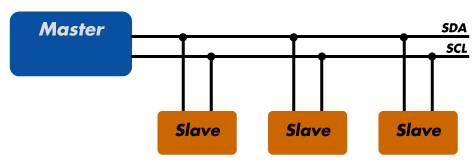
\includegraphics[scale=0.5]{figuras/8.png} 
	\caption{Comunicação I2C}
	\label{Rotulo}
\end{figure}

Os dispositivos ligados em Inter IC possuem um endereço fixo (cada componente recebe um endereço específico), e podemos configurá-los para receber ou transmitir dados; dessa maneira eles podem ser classificados de várias formas, como: mestres (MASTER), escravos (SLAVE), entre outras.\cite{I2C}

O barramento I2C é do tipo multi-mestre, isso significa que mais de um dispositivo de controle pode ser conectado a ele. No entanto, durante uma comunicação, somente um dos mestres pode estar ativo, ou ocorrerá uma colisão de dados no barramento. Dispositivos I2C possuem um endereço que os identifica. Esse endereço é composto normalmente por 7 bits. \cite{I2C}

\begin{figure}[!htb]
	\centering
	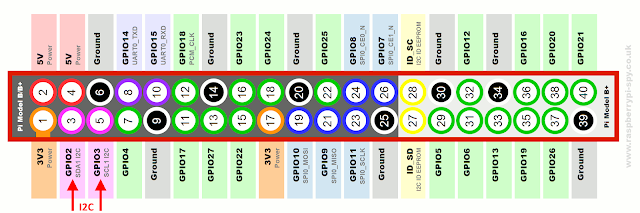
\includegraphics[scale=0.5]{figuras/9.png} 
	\caption{GPIO Raspberry Pi}
	\label{Rotulo}
\end{figure}

O protocolo de comunicação UART,é  assíncrono, ou seja, não existe um sinal de clock para sincronizar o sinal transmitido com o sinal recebido. A UART é um protocolo de comunicação full-duplex, ou seja, a comunicação é realizada ao mesmo tempo de um dispositivo para o outro, pois os dados trafegam por meios diferentes. \cite{UART}

Para os bits serem transmitidos e recebidos,  o sinal transmissor e o sinal receptor devem estar configurados com o mesmo valor, dado em bits por segundo, que é a taxa de transmissão de dados entre um dispositivo a outro. De acordo com o protocolo UART, quando não há dados no barramento ele é colocado em estado \textit{Bus Idle}, mantido em lógico alto.

Quando um dispositivo possui dados para serem transmitidos, primeiro ele envia um bit de inicialização chamado Start Bit, esse bit está em nível lógico baixo. Logo em seguida envia um byte, ou seja, 8 bits de informação. Para finalizar o envio dos dados, envia um bit chamado de Stop Bit que possui nível lógico alto. \cite{UART}

\begin{figure}[!htb]
	\centering
	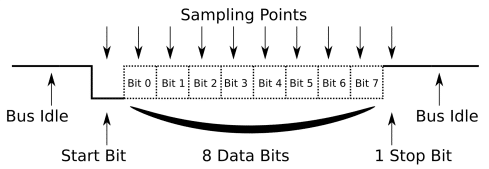
\includegraphics[scale=0.5]{figuras/10.png} 
	\caption{Protocolo UART}
	\label{Rotulo}
\end{figure}

\subsection{Sistema hidrodinâmico}
Para a concepção do sistema hidrodinâmico presente na estufa, foram utilizados um reservatório de água de 15,5 Litros, duas válvulas solenoides de 180 graus 220VAC e sensores de nível água.

\begin{figure}[!htb]
	\centering
	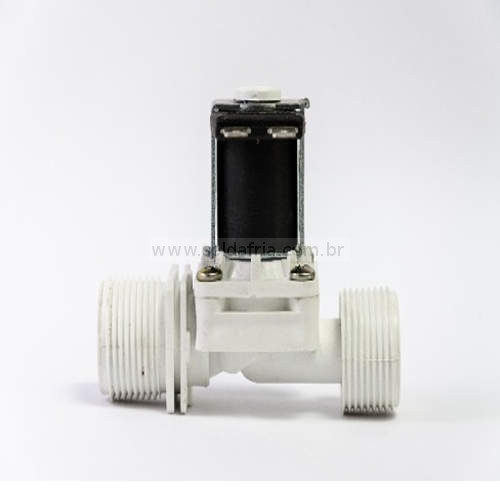
\includegraphics[scale=0.25]{figuras/7.jpg} 
	\caption{Válvula}
	\label{Rotulo}
\end{figure}

\begin{figure}[!htb]
	\centering
	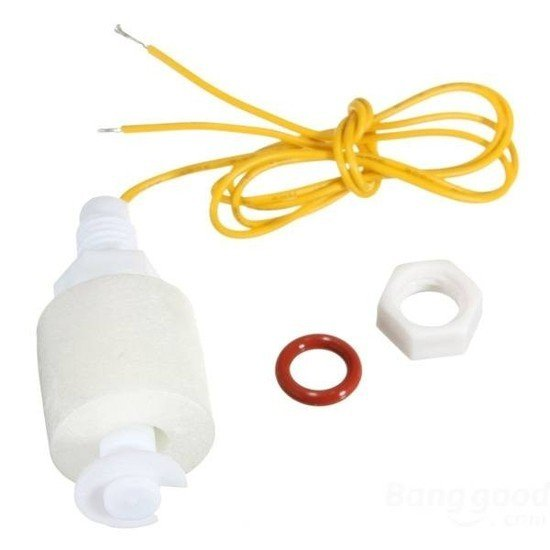
\includegraphics[scale=0.25]{figuras/6.jpg} 
	\caption{Sensor de Nível}
	\label{Rotulo}
\end{figure}

O sistema montado então consiste em uma entrada e saída de água controlada pelas válvulas que são acionadas de acordo com o valor dos sensores de nível de água. Os sensores são dispostos, um na tampa do reservatório, para indicar quando este está cheio e o outro na parte mais profunda do reservatório, indicando quando está com um nível de água baixo.

Os sensores funcionam com uma lógica binaria, porém como são colocados em posições invertidas os sinais que são enviados pelos para a mesma informação são diferentes. Se  o sensor superior estiver detectando água, o seu circuito interno é fechado e um sinal de nível lógico alto é enviado para a Raspberry. O sensor de baixo quando detecta água abre o circuito enviando um sinal de nível lógico baixo para a Raspberry. Com isso, foi feito um sistema de controle para manter o reservatório cheio utilizando os sinais que os sensores de nível enviam e o acionamento das válvulas de entrada e saída de água. 

O sistema é utilizado sempre que a solução nutritiva precisa ser trocada, permitindo assim o usuário realizar uma troca fácil e eficiente evitando que seja necessário a movimentação do reservatório uma vez que as entradas de água são fixas e podem ser conectadas de forma semelhante a conexão realizada em máquinas de lavar roupas.
As válvulas solenoides que compõem o projeto tem uma vazão mínima de 7L/min permitindo assim que o reservatório que contém 15,5L fique completamente cheio em 2 min e 12 segundos, pode-se ainda diminuir o tempo aumentando a vazão de água que passa pela válvula, uma vez que ela tem como especificação uma vazão máxima de 40L/min.

\subsection{Sistema Eletromecânico}

Para a criação do sistema eletromecânico que integra a gaveta, a equipe de Engenharia eletrônica utilizou uma corrediça telescópica de 35cm, junto com uma polia lisa no inicio e uma polia dentada ligada diretamente no motor DC 12V, além de uma correia de impressora HP. \cite{MotorCC}

\begin{figure}[!htb]
	\centering
	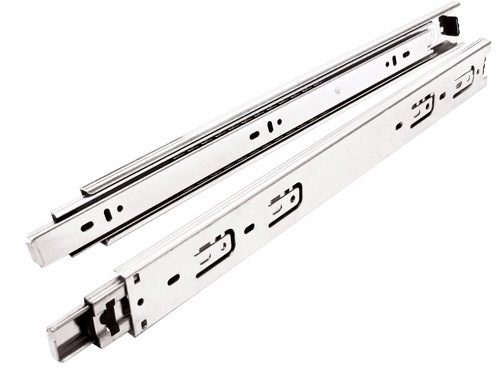
\includegraphics[scale=0.25]{figuras/1.png} 
	\caption{Sistema da Gaveta- Corrediça telescópica}
	\label{Rotulo}
\end{figure}

\begin{figure}[!htb]
	\centering
	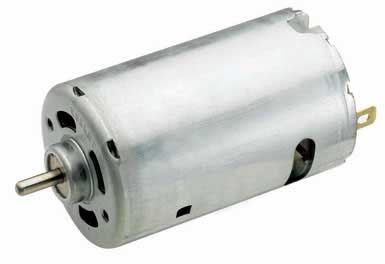
\includegraphics[scale=0.25]{figuras/2.png} 
	\caption{Sistema da Gaveta- Motor 12V DC}
	\label{Rotulo}
\end{figure}

\begin{figure}[!htb]
	\centering
	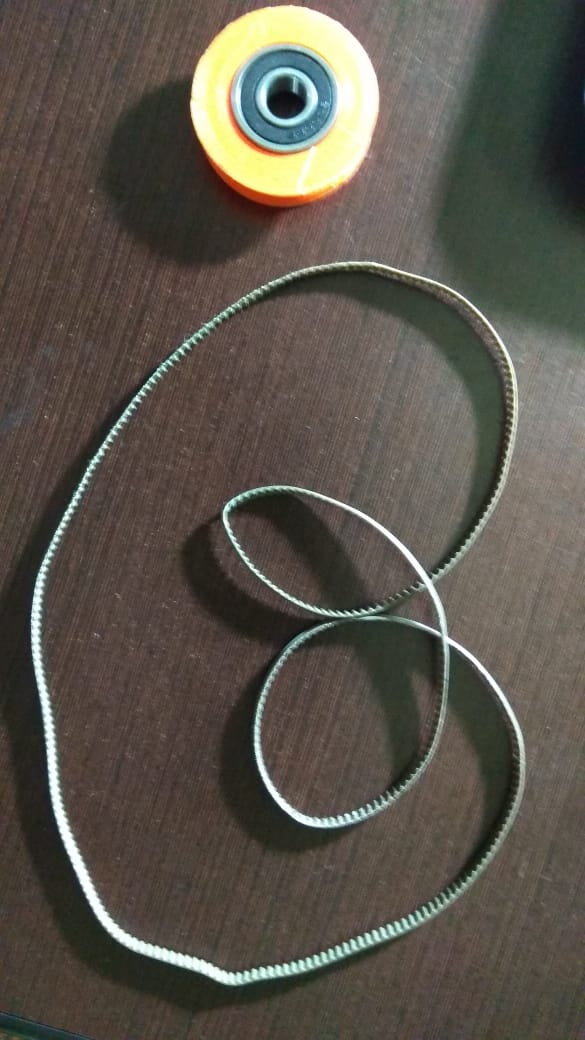
\includegraphics[scale=0.15]{figuras/3.jpeg} 
	\caption{Sistema da Gaveta- polia lisa e correia dentada}
	\label{Rotulo}
\end{figure}

\newpage

Especificações básicas ou primárias para motores DC/CC:

\begin{itemize}
	\item Velocidade
	\item Torque
	\item Tensão
\end{itemize}
Com Tais especificações é possível determinar qual motor dos fabricantes atenderá as necessidades de projeto para realização e execução das etapas usadas no projeto que terá o uso do motor. 

Os Motores CC sem Núcleo e sem ranhura incorporam um enrolamento cilíndrico que está fisicamente fora de um conjunto de ímãs permanentes. Devido ao fato do enrolamento ser laminado e não existir gaiola de ferro, motores cc sem núcleo possuem inércia muito menor. Possuem alta aceleração, eficiência e excelente controle de velocidade com pouca ou nenhuma vibração. Eles são comumente usados como servo motor para aplicações de controle de processo.\cite{EspeciMotorCC}

Os motores elétricos escovados usam escovas de contato que se conectam com o comutador para alimentar o rotor. A construção escovada é menos onerosa do que o motor sem escovas e o controle é mais simples e barato. Outra característica é que o escovado pode operar em ambientes extremos devido à sua ausência interna de componentes eletrônicos. Por outro lado, motores escovados exigem manutenção periódica para substituição das escovas desgastadas.\cite{MotorCC}


\textbf{Velocidade do eixo:}


\begin{equation}
\omega_{rad/s} = \omega_{rpm} \frac{2 \pi}{60} 
\end{equation}
A velocidade deve ser testada variando a tensão do motor sem nenhum tipo de carga sendo acionada pelo mesmo, o motor deve está livre de qualquer grandeza física que dificulte sua rotação.


\textbf{Torque de saída:}

\begin{equation}
\tau = K. l 
\end{equation}

A velocidade de rotação do motor gera uma força, que é definida físicamente como torque, o torque é dado em unidade de força- distância. Podendo ser de duas maneiras: Partida ou torque contínuo. \cite{EspeciMotorCC}

\textbf{Tensão}

Os motores CC são projetados para trabalhar em função de uma corrente contínua, sendo por isso projetados para trabalhar sob uma tensão específica. No caso da aplicação do projeto utilizamos o motor 12 V DC.

Para retirar as varíaveis das quais não tivemos conhecimento prévio, por se tratar de um motor retirado de equipamentos eletrônicos que estavam para reciclagem, o uso de um mediro de tacômetro digital de contato é altamente indicado para o projeto e especificações básicas como RPM.\cite{EspeciMotorCC}


\begin{figure}[!htb]
	\centering
	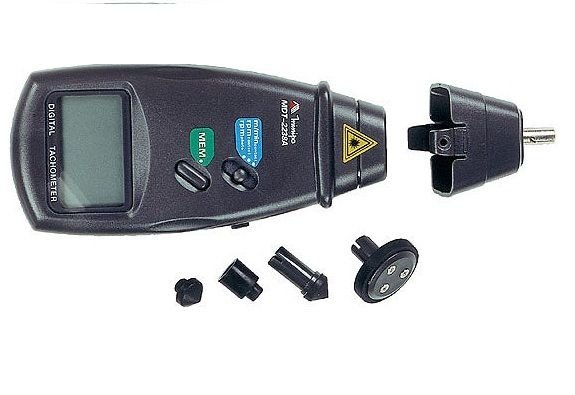
\includegraphics[scale=0.35]{figuras/5.jpg} 
	\caption{Sistema da Gaveta- Tacômetro}
	\label{Rotulo}
\end{figure}

\subsection{Sistema Embarcado}


Para o projeto de sistemas embarcados, mais propriamente o firmware da gaveta,implementou-se uma lógica de estados digital para a abertura e fechamento. As entradas da máquina de estado foram os sensores (\textit{Reed Switchs}), na parte traseira e frontal da gaveta e um sensor para verificar se a porta estava aberta ou fechada, além disso foi acrescentado um botão(\textit{pushbuttom}) para ser utilizado como comando, assim como o sinal vindo da API. As saída da máquina de estado que controla a gaveta, definem o movimento do motor, o qual pode ser parado, sentido anti-horário e horário. E os estados são Abrindo, Aberto, Fechado e Fechando (Figura \ref{maquina_gaveta}).

\begin{figure}[!htb]
	\centering
	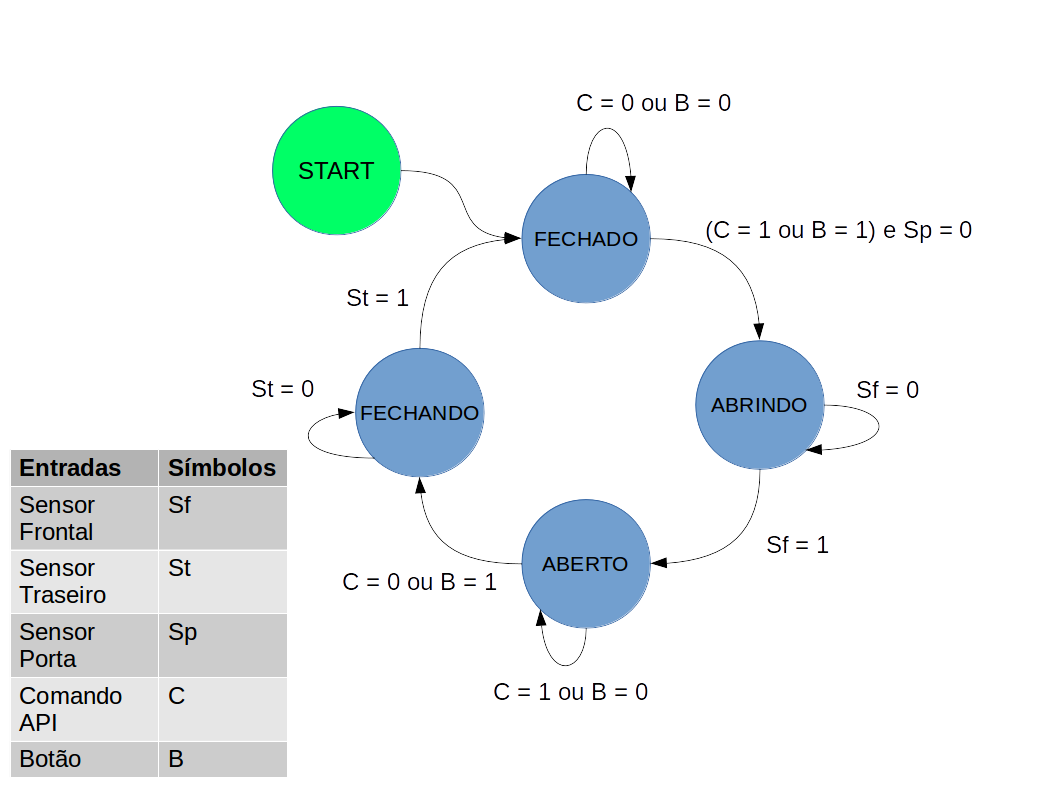
\includegraphics[scale=0.35]{figuras/Maquina_Gaveta.png} 
	\caption{Máquina de estados da gaveta}
	\label{maquina_gaveta}
\end{figure}  

Para o reservatório também existe uma lógica de estados que engloba às válvulas e as bombas d'água de acordo com os estados das bóias. As entradas são os valores das bóias e um comando que vem do API. As saídas definem como se comportarão as bombas e válvulas de entrada e sáida de água. Os estados são vazio, mediano, cheio e esvaziando. Ele só esvazia caso o utilizador envie o comando (Figura \ref{maquina_reservatorio}).

\begin{figure}[!htb]
	\centering
	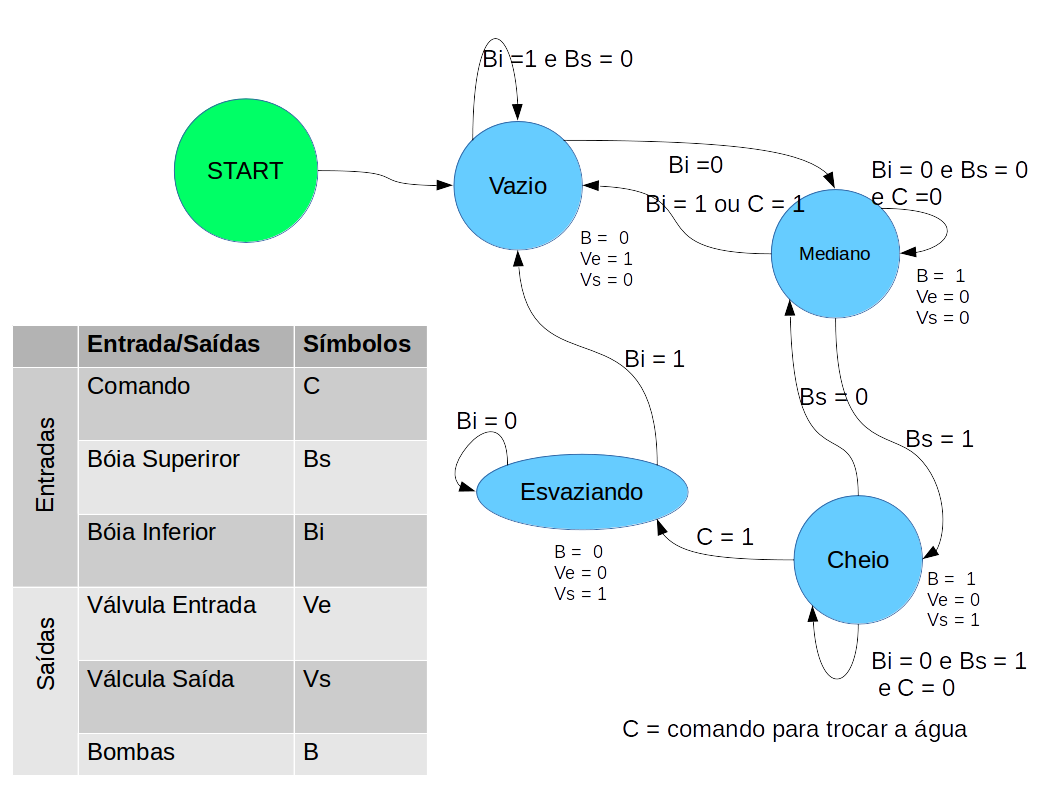
\includegraphics[scale=0.35]{figuras/ControleReservatorio.png} 
	\caption{Máquina de estados do reservatório}
	\label{maquina_reservatorio}
\end{figure} 

\subsection{Pinagem do Sistema na Raspberry Pi 3}

Para o processo de conexão dos pinos na placa Raspberry Pi 3, segue a seguinte tabela de interconexões. E uma descrição a partir de cores de qual a tensão de cada um dos sensores (Figura \ref{pinagem}).


\begin{figure}[!htb]
	\centering
	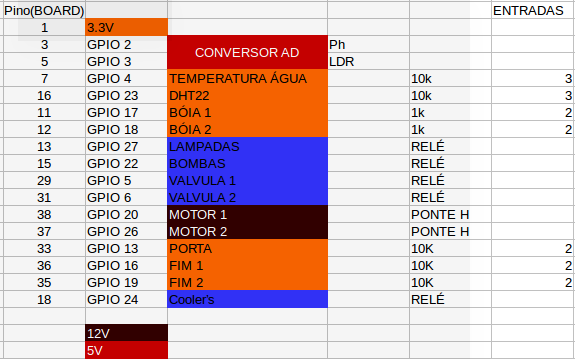
\includegraphics[scale=0.60]{figuras/Pinagem.png} 
	\caption{Pinagem GPIO do Sistema}
	\label{pinagem}
\end{figure} 

\section{Solução Química e suas especificações}

Cada litro de solução é suficiente para a produção de um pé de alface desde a muda, de segunda folha verdadeira, até a colheita, outras hortaliças folhosas de menor porte, como rúcula, consomem menos solução. Em meia a colheita é feita até 45 dias após a inserção da muda na solução hidropônica em definitivo. É necessário sempre manter a condutividade entre 1.000 à 1500 $\mu S/cm$ de concentração total de íons na solução. A temperatura idela para plantas cultivadas em hidropônia está na faixa de 18 a 24 graus celsius no verão e 10 a 16 graus celsius no inverno. As plantas têm seu desenvolvimento máximo entre o pH 5,5 a 6,5.

\subsection{Descrição do produto hidropônico}
Solução para 1000L
\begin{itemize}
	\item 400g de sulfato de magnésio 9\%  multitécnica, garantia mínima de 9\% Mg + 12 \%S
	\item 150g Fosfato monoamônico MAP: Garantia minima de 11\%N + 60\% P2O5
	\item 750g Nitrato de Cálcio garantia mínima de 15,5 \%N + 6\%Ca
	\item 30g Quelato de Ferro, garantia mínima 6\%F + 40,8\% EDDHA
	\item 500g de nitrato de potássio , garantia minima de 52\% de fósforo e 34\% de potássio
	\item 30g de coquetel de micronutrientes 
\end{itemize}

\subsection{Método de dissolulção}

\begin{itemize}
	\item Coloque 7,5L de água no reservatório
	\item Misture a seco o sulfato de magnésio , fosfato monoâmonico, nitrato de potássio
	\item Dissolva essa mistura em um recipiente com água e coloque no reservatório
	\item Dissolva o nitrato de cálcio com água e coloque no reservatório
	\item Dissolva o coquetel de micronutrientes  com água e coloque no reservatório
	\item  Dissolva o ferro quelatizado com água e coloque no reservatório
	\item Toda vez que adicionar um componente no reservatório misture bem
	\item Agora complete até atingir 15 L
\end{itemize}
\subsection{Alteração de pH caso necessário}

Se a leitura do pH estiver na faixa de 5,5 a 6,5 pH, caso contrário

\begin{itemize}
	\item Diminuir o pH: Vinagre Branco
	\item Aumentar o pH: Bicaarbonato de cálcio
\end{itemize}

